\tikzset{every picture/.style={line width=0.75pt}} %set default line width to 0.75pt        

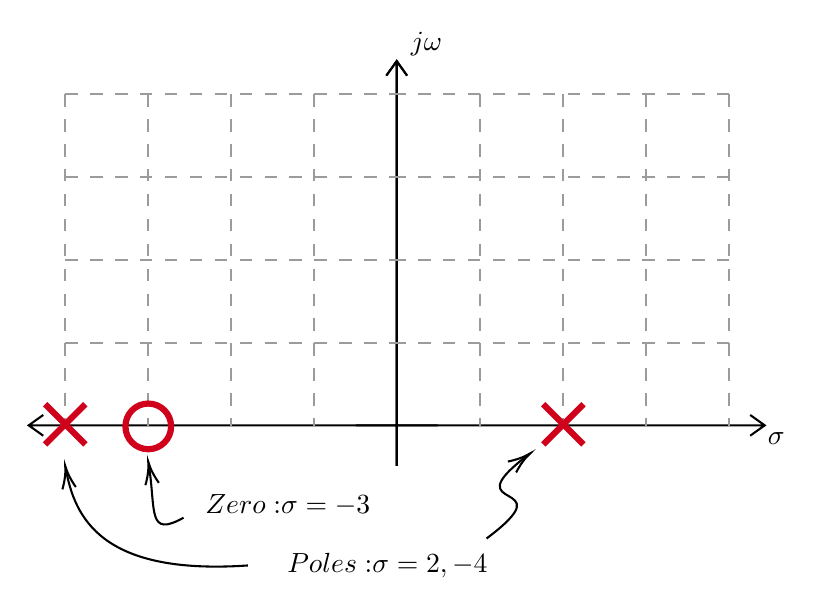
\begin{tikzpicture}[x=0.75pt,y=0.75pt,yscale=-1,xscale=1]
%uncomment if require: \path (0,300); %set diagram left start at 0, and has height of 300

%Shape: Axis 2D [id:dp8113302705977828] 
\draw  (303,209.5) -- (500,209.5)(322.7,34) -- (322.7,229) (493,204.5) -- (500,209.5) -- (493,214.5) (317.7,41) -- (322.7,34) -- (327.7,41)  ;
%Shape: Axis 2D [id:dp36360353813604684] 
\draw  (342.4,209.5) -- (145.4,209.5)(322.7,34) -- (322.7,229) (152.4,204.5) -- (145.4,209.5) -- (152.4,214.5) (327.7,41) -- (322.7,34) -- (317.7,41)  ;
%Shape: Grid [id:dp04715488477638419] 
\draw  [draw opacity=0][dash pattern={on 4.5pt off 4.5pt}] (163,50) -- (323,50) -- (323,210) -- (163,210) -- cycle ; \draw  [color={rgb, 255:red, 155; green, 155; blue, 155 }  ,draw opacity=1 ][dash pattern={on 4.5pt off 4.5pt}] (163,50) -- (163,210)(203,50) -- (203,210)(243,50) -- (243,210)(283,50) -- (283,210) ; \draw  [color={rgb, 255:red, 155; green, 155; blue, 155 }  ,draw opacity=1 ][dash pattern={on 4.5pt off 4.5pt}] (163,50) -- (323,50)(163,90) -- (323,90)(163,130) -- (323,130)(163,170) -- (323,170) ; \draw  [color={rgb, 255:red, 155; green, 155; blue, 155 }  ,draw opacity=1 ][dash pattern={on 4.5pt off 4.5pt}]  ;
%Shape: Grid [id:dp09911761043667966] 
\draw  [draw opacity=0][dash pattern={on 4.5pt off 4.5pt}] (483,50) -- (483,210) -- (323,210) -- (323,50) -- cycle ; \draw  [color={rgb, 255:red, 155; green, 155; blue, 155 }  ,draw opacity=1 ][dash pattern={on 4.5pt off 4.5pt}] (483,50) -- (323,50)(483,90) -- (323,90)(483,130) -- (323,130)(483,170) -- (323,170) ; \draw  [color={rgb, 255:red, 155; green, 155; blue, 155 }  ,draw opacity=1 ][dash pattern={on 4.5pt off 4.5pt}] (483,50) -- (483,210)(443,50) -- (443,210)(403,50) -- (403,210)(363,50) -- (363,210) ; \draw  [color={rgb, 255:red, 155; green, 155; blue, 155 }  ,draw opacity=1 ][dash pattern={on 4.5pt off 4.5pt}]  ;
%Straight Lines [id:da14959838585901308] 
\draw [color={rgb, 255:red, 208; green, 2; blue, 27 }  ,draw opacity=1 ][line width=2.25]    (172.69,199.31) -- (153.31,218.69) ;
%Straight Lines [id:da9187014735355266] 
\draw [color={rgb, 255:red, 208; green, 2; blue, 27 }  ,draw opacity=1 ][line width=2.25]    (172.69,218.69) -- (153.31,199.31) ;

%Straight Lines [id:da34748518935238404] 
\draw [color={rgb, 255:red, 208; green, 2; blue, 27 }  ,draw opacity=1 ][line width=2.25]    (412.69,199.31) -- (393.31,218.69) ;
%Straight Lines [id:da12270667926777268] 
\draw [color={rgb, 255:red, 208; green, 2; blue, 27 }  ,draw opacity=1 ][line width=2.25]    (412.69,218.69) -- (393.31,199.31) ;

%Shape: Circle [id:dp9300460151745538] 
\draw  [color={rgb, 255:red, 208; green, 2; blue, 27 }  ,draw opacity=1 ][line width=2.25]  (192,210) .. controls (192,203.92) and (196.92,199) .. (203,199) .. controls (209.08,199) and (214,203.92) .. (214,210) .. controls (214,216.08) and (209.08,221) .. (203,221) .. controls (196.92,221) and (192,216.08) .. (192,210) -- cycle ;
%Curve Lines [id:da5007254328073322] 
\draw    (366,264) .. controls (405.6,234.3) and (348.17,252.62) .. (385.83,223.89) ;
\draw [shift={(387,223)}, rotate = 143.13] [color={rgb, 255:red, 0; green, 0; blue, 0 }  ][line width=0.75]    (10.93,-3.29) .. controls (6.95,-1.4) and (3.31,-0.3) .. (0,0) .. controls (3.31,0.3) and (6.95,1.4) .. (10.93,3.29)   ;
%Curve Lines [id:da11812747973336613] 
\draw    (251,277) .. controls (179.82,281.88) and (167.59,253.48) .. (163.31,230.74) ;
\draw [shift={(163,229)}, rotate = 80.13] [color={rgb, 255:red, 0; green, 0; blue, 0 }  ][line width=0.75]    (10.93,-3.29) .. controls (6.95,-1.4) and (3.31,-0.3) .. (0,0) .. controls (3.31,0.3) and (6.95,1.4) .. (10.93,3.29)   ;
%Curve Lines [id:da6924425384299892] 
\draw    (220,254) .. controls (202.45,263.75) and (206.76,250.68) .. (203.28,228.71) ;
\draw [shift={(203,227)}, rotate = 80.13] [color={rgb, 255:red, 0; green, 0; blue, 0 }  ][line width=0.75]    (10.93,-3.29) .. controls (6.95,-1.4) and (3.31,-0.3) .. (0,0) .. controls (3.31,0.3) and (6.95,1.4) .. (10.93,3.29)   ;

% Text Node
\draw (500,211.4) node [anchor=north west][inner sep=0.75pt]    {$\sigma $};
% Text Node
\draw (328,18.4) node [anchor=north west][inner sep=0.75pt]    {$j\omega $};
% Text Node
\draw (318.24,269.4) node [anchor=north] [inner sep=0.75pt]    {$\text{Poles: } \sigma =2,-4$};
% Text Node
\draw (229,241.4) node [anchor=north west][inner sep=0.75pt]    {$\text{Zero: } \sigma =-3$};


\end{tikzpicture}
